\documentclass[../main]{subfile}
\graphicspath{{\subfix{../images}}}
\begin{document}

近来,候选区域生成方法和基于区域的卷积神经网络的成功驱动了物体检测的进步(例如,\cite{selectiveSearch})。虽然在最初开发的\cite{rcnn}中基于区域的CNN是计算昂贵的,但是由于候选区域间的卷积共享,使得它们的开销被显著降低。最近的版本,Fast R-CNN\cite{fastrcnn}使用非常深的网络,\textit{在忽略候选区域生成的情况下},几乎实现了实时速率。如今,候选区域生成是最优检测系统的测试时间计算瓶颈。

候选区域生成方法通常依赖于不昂贵的特征以及经济的推理策略。选择搜索\cite{selectiveSearch},其中一种最流行的方法,基于设计好的低层次特征贪心地合并超像素。然而与高效的检测网络\cite{fastrcnn}相比,选择搜索比之慢一个数量级,在CPU实现中处理每个图片需要2秒。EdgeBoxes\cite{edgeBoxes}目前提供了候选区域质量和速度间的最好平衡,处理每张图片的速度达到了0.2秒。然而,候选区域生成步骤仍然和检测网络花费了相同的运行时间。

人们可能会注意到fast R-CNN借用了GPU的优势,然而候选区域生成方法是在CPU上实现的,这使得运行时间的比较并不公平。加速候选计算的一个显然方法便是为了GPU重新实现它。这可能是一个有效的工程解决方法,但是重新实现忽视了下游的检测网络并因此忽视了共享计算的重要机会。

在这片文章中,我们展示了一种算法方面的改变,使用深度卷积神经网络来计算候选区域,这引领了一种优雅且有效的解决方式——。给了检测网络的计算,候选计算几乎是免费的。作为结尾,我们提出了一个新的可以和最好的物体检测网络\cite{fastrcnn, rcnn}共享卷基层的\textit{候选区域生成网络}(RPN)。通过在测试时共享卷积,计算候选区域的额外开销很小(例如,每张图10毫秒)。

我们的发现是基于区域的检测器,例如Fast R-CNN,使用的卷积特征图,也可以被用来生成候选区域。在这些卷积特征的上面,我们通过额外加入一些在常规网格的每个位置同时回归区域边界和置信度的卷积层的方式,构建了一个RPN。RPN因此是一种全卷积网络(FCN)\cite{fcn}并可以针对生成检测候选区域任务端到端训练。

\begin{figure}[bh]
    \centering
    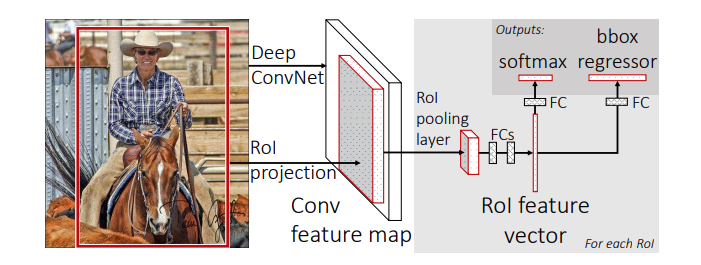
\includegraphics[width=.8\textwidth]{fig1.png}
    \label{fig:img1}
    \caption{解决多尺度和大小的不同方案。(a)构建图片和特征图金字塔,并在所有尺度运行分类器。(b)在特征图上运行多尺度/大小的过滤器。(c)我们在回归函数中使用参考框金字塔。}
\end{figure}

RPN被设计来高效地在广大的尺度范围以及高宽比范围预测候选区域。与之前使用图片金字塔(\ref{fig:img1}, a)或过滤器金字塔(\ref{fig:img1}, b)的流行方法\cite{overfeat, dpm, rcnn, fastrcnn, }相比,我们提出了全新的“锚”框来作为多尺度以及多高宽比的参照(\ref{fig:img1}, c)。我们的方案可以被视为回归参照金字塔,这避免了枚举多个尺度和高宽比的图片或过滤器。当使用单一尺度图片进行训练和测试时,这个模型性能良好,因此对运行速度有益。

为了统一RPN和Fast R-CNN\cite{fastrcnn}物体检测网络,我们提出了一种候选区域生成任务微调和物体检测微调(保持候选固定)交替进行的训练方案。这个方案可以快速收敛并产生一个可以使得两个任务共享卷积特征的统一网络。

我们在PASCAL VOC检测基准上全面地评估了我们的方法,RPN的Fast R-CNN方法得到的检测准确率好于选择搜索的Fast R-CNN。同时,我们的方法几乎消除了测试阶段选择搜索带来的所有计算负担——候选区域生成运行的有效时间仅仅是10毫秒。在使用昂贵的很深的模型\cite{vgg}的情况下,我们的检测方法依旧在单块GPU上达到了5fps的速率(\textit{包含所有步骤}),因此这是就速度和准确率而言的实际物体检测系统。我们也汇报了在MS COCO数据集上的结果并探讨了使用MS COCO的数据提高在PASCAL VOC上的表现。数据已经在\href{https://github.com/shaoqingren/faster\_rcnn}{https://github.com/shaoqingren/faster\_rcnn}(MATLAB版本)和\href{https://github.com/rbgirshick/py-faster-rcnn}{https://github.com/rbgirshick/py-faster-rcnn}(Python版本)开源。

这个手稿的早期版本在之前已经发表。在那之后,RPN和Faster R-CNN框架被采用并推广到其他方法,例如三维物体检测\cite{3dCase},基于部分的检测\cite{partCase},实例分割\cite{segCase}和图片字幕。我们的快速并有效的物体检测系统也在汇报了用户参与度改进的情况下,在例如Pinterests的商业系统中被构建。

在ILSVRC和COCO 2015竞赛中,Faster R-CNN和RPN是在ImageNet检测,ImageNet定位,COCO检测和COCO分割的多个赛道中多个第一名条目的基础。RPN王权从数据中学习生成候选区域,因此可以轻易从更深以及更有表达性的特征(例如在\cite{resnet}中采用的101层残差网络)中受益。Faster R-CNN和RPN也在那些竞赛中的领先条目中被使用。这些结果表明我们的方法不仅是对实际用法开销高效的方法,同时也是一种提升物体检测准确率的有效方式。

\end{document}